\documentclass{article}

% NeurIPS 2026 workshop style (self-contained approximation)
\usepackage[utf8]{inputenc}
\usepackage[T1]{fontenc}
\usepackage{microtype}
\usepackage[numbers,sort&compress]{natbib}
\usepackage{hyperref}
\usepackage{url}
\usepackage{booktabs}
\usepackage{amsfonts}
\usepackage{amsmath}
\usepackage{amssymb}
\usepackage{nicefrac}
\usepackage{xspace}
\usepackage{graphicx}
\usepackage{subcaption}
\usepackage{xcolor}
\usepackage{multirow}
\usepackage{tikz}
\usetikzlibrary{arrows.meta, positioning, fit, backgrounds, shapes.geometric}

% Page geometry (NeurIPS workshop: letter, 1in margins)
\usepackage[letterpaper, margin=1in]{geometry}

% NeurIPS-style font
\usepackage{times}

% Paragraph spacing
\setlength{\parskip}{0pt}
\setlength{\parindent}{1em}

% Compact section spacing
\usepackage{titlesec}
\titlespacing*{\section}{0pt}{8pt plus 2pt minus 2pt}{4pt plus 1pt minus 1pt}
\titlespacing*{\subsection}{0pt}{6pt plus 2pt minus 2pt}{3pt plus 1pt minus 1pt}

\newcommand{\PCSP}{\textsc{pcsp}}
\newcommand{\eg}{\textit{e.g.}\xspace}
\newcommand{\ie}{\textit{i.e.}\xspace}
\newcommand{\etal}{\textit{et al.}\xspace}

% ---------------------------------------------------------------
\title{\textbf{One Policy, Infinite NPCs:}\\
LLM-Persona Conditioned RL for Life Simulation Game NPCs}

\author{
  Anonymous Author(s)\\
  \texttt{anonymous@institution.edu}
}

\date{}

\begin{document}
\maketitle

% ---------------------------------------------------------------
\begin{abstract}
We present \PCSP{} (\textbf{P}ersona-\textbf{C}onditioned \textbf{S}hared \textbf{P}olicy),
a framework that enables a single reinforcement learning policy to generate
persona-consistent, behaviorally diverse NPC behaviors from free-form natural
language persona descriptions.
\PCSP{} encodes persona text with a frozen LLM (Qwen3-0.6B-Embedding) plus a
learned LoRA projection, then conditions a lightweight policy network via
FiLM (\textbf{F}eature-wise \textbf{L}inear \textbf{M}odulation) at every hidden
layer.
Training combines standard PPO with two auxiliary objectives: an InfoNCE-based
\textit{consistency loss} that forces trajectories to be traceable back to their
persona, and a KL-based \textit{diversity loss} that prevents behavioral collapse.
On our \textit{Mini-Inzoi} life-simulation benchmark (6$\times$6 grid, 4 agents,
8 needs, 300 personas),
\PCSP{} achieves zero-shot persona generalization on 60 unseen personas
with trajectory-to-persona identification 11$\times$ above chance
(19.3\% vs.\ 1.7\% random),
Spearman $\rho\!=\!0.73$ between embedding distance and behavioral KL divergence,
and 22$\times$ faster inference than LLM-as-policy (1.97\,ms vs.\ 43.7\,ms).
Ablation studies confirm that FiLM conditioning, LoRA projection, and both
auxiliary losses are each individually necessary.
\end{abstract}

% ---------------------------------------------------------------
\section{Introduction}
\label{sec:intro}

Life simulation games such as \textit{The Sims} and \textit{inZOI} demand
\emph{hundreds to thousands} of NPCs that each behave consistently with a
distinct personality---across an entire play session, not just in a single
dialogue.
Industrial solutions today rely on hand-crafted behavior trees, whose authoring
cost scales with the NPC count, or fall back to generic stochastic policies
that produce no consistent character.

Two natural alternatives face hard scaling walls.
\emph{One-policy-per-persona RL} requires memory and training cost linear in the
number of NPCs; deploying 10{,}000 distinct policies is impractical.
\emph{LLM-as-policy} methods~\citep{ahn2022saycan,wang2023voyager} achieve
expressive persona conditioning but call the language model at every step,
incurring 200--500\,ms latency that conflicts with real-time game loops (target:
$<$50\,ms).

We propose \PCSP{} to close this gap.
The key insight is that a frozen LLM encoder computes a \emph{once-per-NPC}
persona embedding; a lightweight FiLM-conditioned policy network then runs at
full game speed.
The shared policy generalizes to unseen persona texts through the smooth semantic
structure of LLM embedding space.

\paragraph{Contributions.}
\begin{enumerate}
  \setlength\itemsep{0pt}
  \item \textbf{\PCSP{} framework}: a single shared RL policy conditioned on
    LLM persona embeddings via FiLM, supporting unlimited NPCs at constant
    inference cost.
  \item \textbf{Co-training objective}: joint PPO + InfoNCE consistency +
    KL diversity loss that prevents behavioral collapse without sacrificing
    task reward.
  \item \textbf{Zero-shot generalization}: $11\times$ above-chance
    trajectory-to-persona identification on 60 unseen personas, with
    Spearman $\rho\!=\!0.73$ semantic-behavioral alignment.
  \item \textbf{Speed advantage}: 22$\times$ faster than LLM-as-policy while
    maintaining interpretable persona conditioning.
\end{enumerate}

% ---------------------------------------------------------------
\section{Related Work}
\label{sec:related}

\paragraph{Goal-conditioned RL.}
UVFA~\citep{schaul2015uvfa} and HER~\citep{andrychowicz2017her} condition
policies on \emph{goal states}---what to achieve.
Persona describes \emph{how to behave}: two NPCs with the same needs but
different personalities should fulfil them via different activity sequences.
This distinction renders goal-conditioning ill-suited for NPC characterization.

\paragraph{Language-conditioned RL.}
BabyAI~\citep{chevalier2019babyai} and LangSAC~\citep{shao2021langsac}
condition on short-horizon natural-language \emph{instructions} that change
episode-by-episode.
\PCSP{} instead conditions on \emph{persistent personality traits}---a
fundamentally different temporal regime where the conditioning signal is fixed
for the NPC's lifetime.

\paragraph{Skill discovery.}
DIAYN~\citep{eysenbach2018diayn} and CIC~\citep{laskin2022cic} discover
diverse skills via unsupervised latent codes.
Learned skills are not human-interpretable; a game designer cannot say
``make this NPC introverted'' by specifying a latent index.
\PCSP{} grounds conditioning directly in natural language, preserving
interpretability.

\paragraph{LLM-as-policy.}
SayCan~\citep{ahn2022saycan}, Voyager~\citep{wang2023voyager}, and
ReAct~\citep{yao2023react} invoke LLMs at \emph{every decision step},
which produces rich persona expression but at latencies ($>$200\,ms)
incompatible with real-time game NPCs.
\PCSP{} calls the LLM once per NPC lifetime.

Table~\ref{tab:related} summarizes the comparison.

\begin{table}[h]
\centering
\small
\caption{Comparison of related paradigms. \PCSP{} is the only approach satisfying
all four desiderata. \checkmark\,= yes, $\times$ = no, $\triangle$ = partial.}
\label{tab:related}
\setlength{\tabcolsep}{5pt}
\begin{tabular}{lcccc}
\toprule
Method & Persona consist. & NL grounding & Zero-shot gen. & Fast ($<$5\,ms) \\
\midrule
Goal-cond RL (UVFA)      & $\times$ & $\times$ & $\times$ & \checkmark \\
Lang-cond RL (BabyAI)    & $\triangle$ & \checkmark & $\triangle$ & \checkmark \\
Skill discovery (DIAYN)  & $\triangle$ & $\times$ & $\times$ & \checkmark \\
Per-NPC RL               & \checkmark & $\times$ & $\times$ & \checkmark \\
LLM-as-policy (SayCan)   & \checkmark & \checkmark & \checkmark & $\times$ \\
\textbf{\PCSP{} (ours)}  & \checkmark & \checkmark & \checkmark & \checkmark \\
\bottomrule
\end{tabular}
\end{table}

% ---------------------------------------------------------------
\section{Method}
\label{sec:method}

\subsection{Environment: Mini-Inzoi}
\label{sec:env}

\textit{Mini-Inzoi} is a PettingZoo AEC life-simulation environment on a
6$\times$6 grid with 4 agents, 8 bio/social needs (hunger, sleep, social,
leisure, hygiene, fitness, work, learning), and 12 discrete actions
(8 activities + 4 movement directions).
Observation $s\!\in\!\mathbb{R}^{20}$: agent position (2), time-of-day (1),
current needs (8), and summaries of the three other agents (9).
Reward combines needs satisfaction, persona-aligned activity bonuses
($+0.5$ per preferred action), and social interaction bonuses
($0.2\!+\!0.3\!\times\!\cos\!\text{-sim}(\text{Big Five}_i, \text{Big Five}_j)$).
Persona dataset: 300 texts generated from 15 Big Five archetypes $\times$ 20
occupations; split 240 train / 60 test (zero-shot).

\subsection{Persona Encoding}
\label{sec:encoding}

Given persona text $p$, we compute a frozen LLM embedding
$\hat{e}_p = f_{\text{LLM}}(p) \in \mathbb{R}^{1024}$ using
Qwen3-0.6B-Embedding~\citep{qwen3embed} (last-token pooling, L2-normalized).
This is computed once per NPC; at 14.6\,ms/persona it is negligible.
A learned LoRA projection~\citep{hu2022lora} ($r\!=\!16$, $\text{lr}\!=\!10^{-4}$)
maps $\hat{e}_p \to e_p \in \mathbb{R}^{64}$:
\[
  e_p = W_{\text{down}}^{\top} \sigma\!\left(W_{\text{up}}^{\top} \hat{e}_p\right),
\]
where $W_{\text{up}} \in \mathbb{R}^{1024\times 512}$ and
$W_{\text{down}} \in \mathbb{R}^{512\times 64}$.
The projection is necessary because raw Qwen3 embeddings capture occupational
similarity more strongly than personality similarity
(salesperson$\leftrightarrow$executive: 0.61 vs.\ trainer$\leftrightarrow$blogger: 0.33).

\subsection{FiLM-Conditioned Policy}
\label{sec:film}

The shared policy $\pi_\theta(a \mid s, e_p)$ is a 3-layer MLP (256-256-10)
where each hidden layer $h_\ell$ is modulated by a FiLM layer:
\[
  h_\ell' = \gamma_\ell(e_p) \odot h_\ell + \beta_\ell(e_p),
\]
with $\gamma_\ell, \beta_\ell\!: \mathbb{R}^{64} \to \mathbb{R}^{256}$ being
small linear networks.
FiLM injects persona information at \emph{every} hidden layer, preventing
the persona signal from being diluted in deep representations.
A separate FiLM-conditioned value network $V_\phi(s, e_p)$ is used for the
critic.
Total trainable parameters: 207K (excluding the frozen LLM).

\subsection{Co-Training Objective}
\label{sec:objective}

We train with a three-term objective:
\begin{equation}
  \mathcal{L}_{\text{total}} = \mathcal{L}_{\text{PPO}}
  + \lambda_1 \mathcal{L}_{\text{consist}}
  + \lambda_2 \mathcal{L}_{\text{diverse}},
\end{equation}
with $\lambda_1\!=\!0.5$, $\lambda_2\!=\!0.1$.

\paragraph{PPO loss.}
Standard clipped surrogate objective with GAE ($\gamma\!=\!0.99$,
$\lambda_{\text{GAE}}\!=\!0.95$, $\epsilon\!=\!0.2$, batch\,$=\!2048$).

\paragraph{Consistency loss.}
A 2-layer GRU trajectory encoder $g_\phi(\tau) \in \mathbb{R}^{64}$
(hidden\,$=\!128$) maps episode trajectories to embeddings.
InfoNCE contrastive loss~\citep{oord2018cpc} (temperature $T\!=\!0.07$)
aligns trajectory embeddings with their originating persona embeddings:
\begin{equation}
  \mathcal{L}_{\text{consist}} = -\log
  \frac{\exp\!\left(\tfrac{\text{sim}(g_\phi(\tau),\, e_p)}{T}\right)}
       {\sum_{p' \in \mathcal{B}} \exp\!\left(\tfrac{\text{sim}(g_\phi(\tau),\, e_{p'})}{T}\right)}.
\end{equation}
This loss prevents the policy from ignoring persona conditioning
(\ie mode collapse).

\paragraph{Diversity loss.}
We maximize the expected KL divergence between the policy distributions
induced by different personas at shared states:
\begin{equation}
  \mathcal{L}_{\text{diverse}} = -\mathbb{E}_{s,\, p \neq p'}\!\left[
    D_{\mathrm{KL}}\!\left(\pi_\theta(\cdot \mid s, e_p)
    \;\|\; \pi_\theta(\cdot \mid s, e_{p'})\right)
  \right].
\end{equation}
This is computed as a batched forward pass over $n\!=\!8$ sampled personas at
32 sampled states per update.

A system overview is shown in Figure~\ref{fig:system}.

\begin{figure}[t]
  \centering
  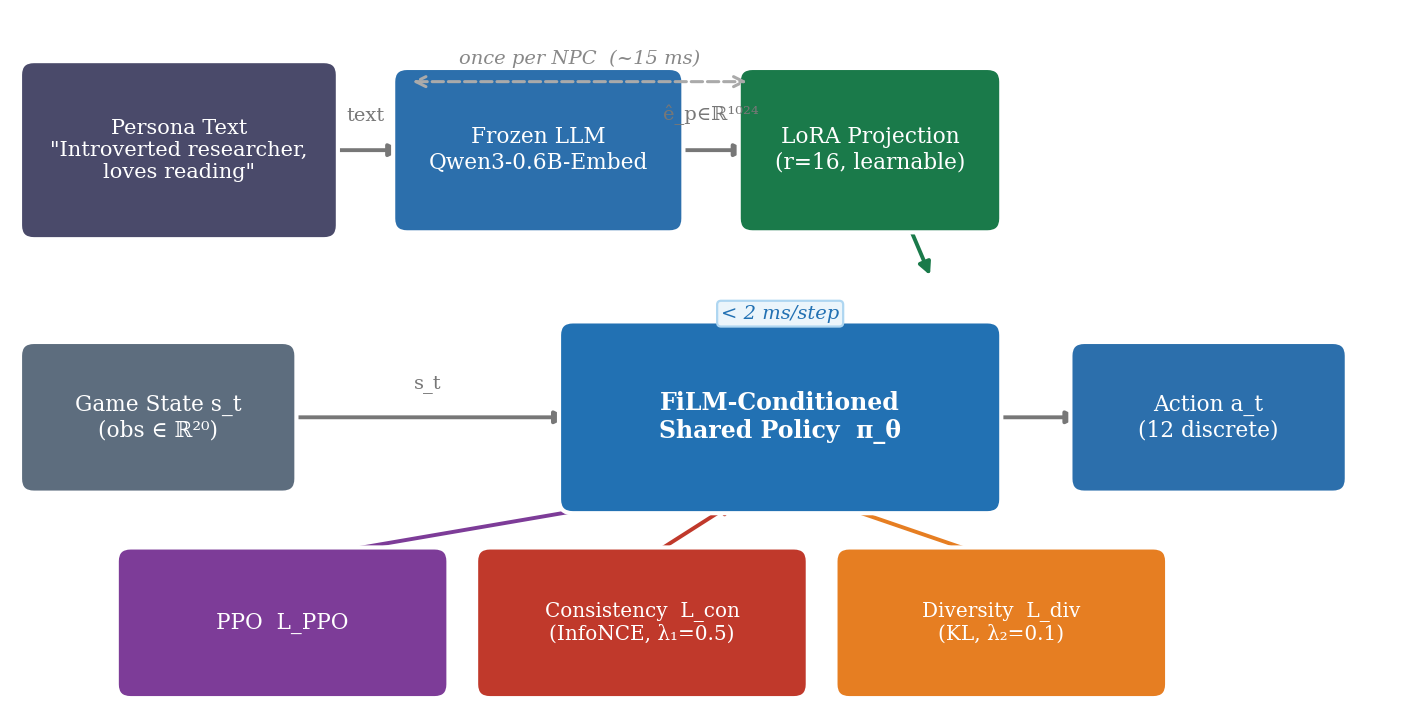
\includegraphics[width=0.92\linewidth]{figures/fig1_system.png}
  \caption{
    \textbf{\PCSP{} system overview.}
    A frozen LLM encoder computes a once-per-NPC persona embedding.
    A learned LoRA projection adapts the embedding to behavior space.
    The shared FiLM-conditioned policy runs at game speed ($<$2\,ms/step)
    and is trained with PPO + consistency + diversity co-objectives.
  }
  \label{fig:system}
\end{figure}

% ---------------------------------------------------------------
\section{Experiments}
\label{sec:experiments}

\subsection{Setup}
\label{sec:setup}

All models are trained for 300 PPO iterations ($\approx$1.9M environment steps)
on an NVIDIA RTX 6000 Ada (49\,GB VRAM).
The \textsc{pcsp} full model trains in approximately 20 minutes.
Baselines:
\textbf{B1} No-Persona PPO (persona-free lower bound);
\textbf{B2} Per-Persona PPO (24 independent policies, data-efficiency upper-bound attempt);
\textbf{B3} SBERT (all-MiniLM-L6-v2, 384-dim, frozen);
\textbf{B4} DIAYN (random 64-dim latent, same FiLM architecture);
\textbf{B5} LLM-as-policy (Qwen3-1.7B, \texttt{/no\_think} mode, latency only).

\subsection{Main Results}
\label{sec:main}

Table~\ref{tab:main} shows per-model results on the five primary metrics.
\PCSP{} (full) achieves the best balance across persona consistency,
zero-shot generalization, behavioral diversity, and inference speed.
While B3 (SBERT) achieves slightly higher task reward (86.2 vs.\ 83.4),
it provides no persona consistency or diversity metrics.

\begin{table}[t]
\centering
\small
\caption{
  \textbf{Main results.}
  Consist.\ Acc: $k$-NN trajectory-to-persona accuracy (train personas).
  ZS Acc / Coh.: $k$-NN accuracy and intra/inter cosine ratio on 60 unseen personas.
  KL: mean pairwise behavioral KL divergence.
  $\rho$: Spearman correlation (embedding distance vs.\ KL).
  Lat.: GPU ms/step (batch~1).
  $^\dagger$KL too small (0.39) for meaningful $\rho$.
}
\label{tab:main}
\setlength{\tabcolsep}{4pt}
\begin{tabular}{lrrrrrrr}
\toprule
Model
  & Reward $\uparrow$
  & Consist.\ Acc $\uparrow$
  & ZS Acc $\uparrow$
  & Coh.\ $\uparrow$
  & KL $\uparrow$
  & $\rho$ $\uparrow$
  & Lat.\ $\downarrow$ \\
\midrule
\textbf{\PCSP{} (full)}
  & 83.4 & 0.283 & 0.193 & 6.24 & 5.87 & \textbf{0.728} & 1.97 \\
PCSP (no\_consist)
  & \textbf{84.3} & 0.008* & 0.017* & 1.04* & 3.78 & 0.638 & 2.03 \\
PCSP (no\_diverse)
  & 76.8 & 0.225 & 0.147 & 4.31 & 0.39* & 0.928\textsuperscript{$\dagger$} & 1.79 \\
PCSP (concat)
  & 77.4 & \textbf{0.392} & \textbf{0.320} & \textbf{8.27} & 2.87 & 0.738 & 1.72 \\
PCSP (frozen\_proj)
  & 83.6 & 0.188 & 0.207 & 2.55 & 5.60 & 0.384 & 1.79 \\
\midrule
B1 No-Persona & 73.2 & {---} & {---} & {---} & {---} & {---} & 1.83 \\
B3 SBERT      & 86.2 & {---} & {---} & {---} & {---} & {---} & 1.88 \\
B4 DIAYN      & 81.9 & {---} & {---} & {---} & {---} & {---} & 1.94 \\
B5 LLM-policy & {---} & {---} & {---} & {---} & {---} & {---} & 43.7 \\
\bottomrule
\end{tabular}
{\footnotesize * Near-random, indicating failure mode.}
\end{table}

\subsection{Ablation Analysis}
\label{sec:ablation}

\begin{figure}[t]
  \centering
  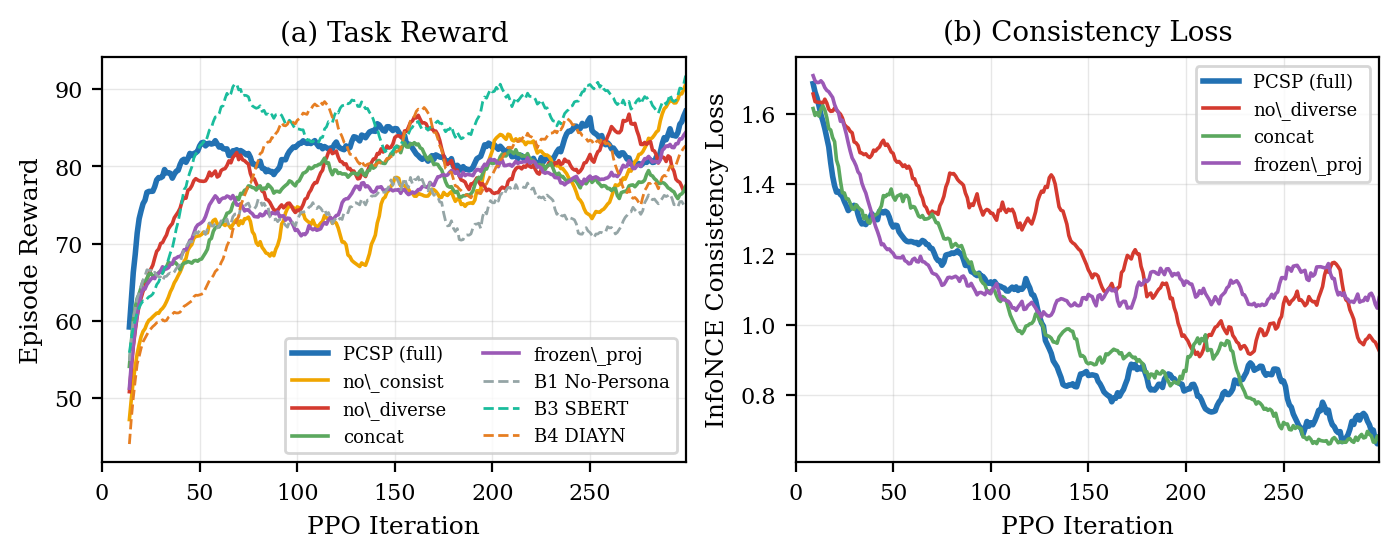
\includegraphics[width=0.96\linewidth]{figures/fig2_learning_curves.png}
  \caption{
    \textbf{Learning curves.}
    (a) Episode reward for \PCSP{} variants and baselines.
    (b) InfoNCE consistency loss during training.
    Removing the consistency loss (\texttt{no\_consist}) prevents the loss from
    converging and causes trajectory embeddings to carry no persona information.
  }
  \label{fig:learning_curves}
\end{figure}

Figure~\ref{fig:learning_curves} shows reward and consistency loss curves
throughout training.

\paragraph{Consistency loss is necessary for persona traceability.}
Removing it (no\_consist) drives consistency accuracy to near-chance (0.8\%,
$11\times$ below full) and zero-shot accuracy to 1.7\%---trajectories carry
no persona information.
The coherence ratio collapses from 6.24 to 1.04, confirming that without this
loss all personas produce nearly identical trajectory embeddings.

\paragraph{Diversity loss is necessary for behavioral differentiation.}
Removing it (no\_diverse) reduces mean KL from 5.87 to 0.39 (15$\times$
reduction), meaning all personas converge to near-identical action
distributions.
Task reward also drops ($-8.5\%$), suggesting that behavioral diversity
improves the policy's ability to satisfy different needs profiles.

\paragraph{FiLM outperforms concatenation in behavioral diversity.}
The concat variant achieves higher consistency accuracy (0.392 vs.\ 0.283)
and coherence (8.27 vs.\ 6.24), but at the cost of task reward
($-7.0\%$) and mean KL ($-51\%$).
The concat architecture exposes persona information only at the input,
limiting its effect on deeper representations and collapsing behavioral range.

\paragraph{LoRA projection aligns semantic structure.}
Freezing the projection (frozen\_proj) halves Spearman $\rho$
(0.384 vs.\ 0.728), indicating that raw LLM embeddings---which capture
occupational similarity more than personality similarity---are not directly
suited for behavior conditioning.

\subsection{Zero-Shot Generalization}
\label{sec:zeroshot}

\begin{figure}[t]
  \centering
  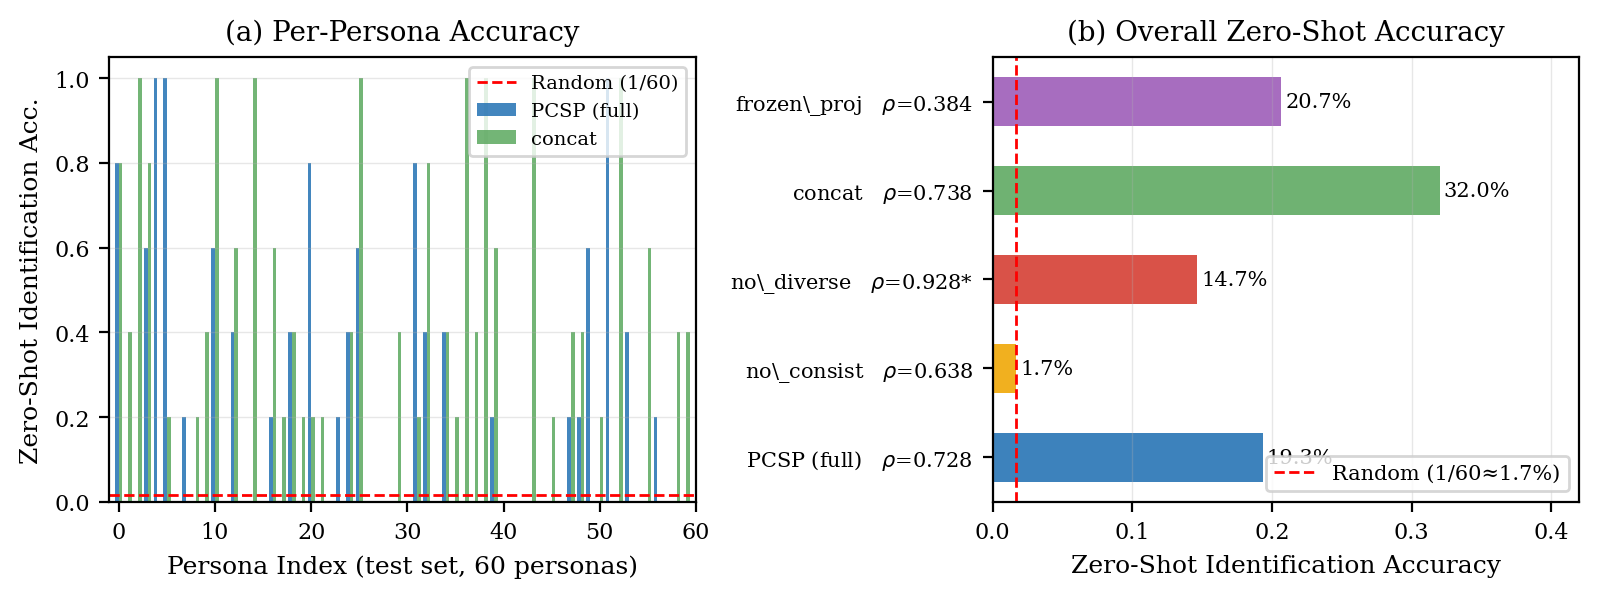
\includegraphics[width=0.96\linewidth]{figures/fig4_zeroshot.png}
  \caption{
    \textbf{Zero-shot generalization on 60 unseen personas.}
    (a) Per-persona identification accuracy for \PCSP{} (full) and concat.
    (b) Overall zero-shot accuracy across all ablations.
    The red dashed line marks random-chance (1/60 $\approx$ 1.7\%).
    \PCSP{} (full) achieves 19.3\%, an 11$\times$ improvement.
  }
  \label{fig:zeroshot}
\end{figure}

Figure~\ref{fig:zeroshot} shows the per-persona zero-shot identification
accuracy for \PCSP{} (full) and the concat ablation across the 60 held-out
personas.
\PCSP{} identifies 19.3\% of unseen personas correctly
(random baseline: 1.7\%), confirming that the LLM embedding space generalizes
to persona texts unseen during training.

\subsection{Semantic--Behavioral Alignment}
\label{sec:alignment}

\begin{figure}[t]
  \centering
  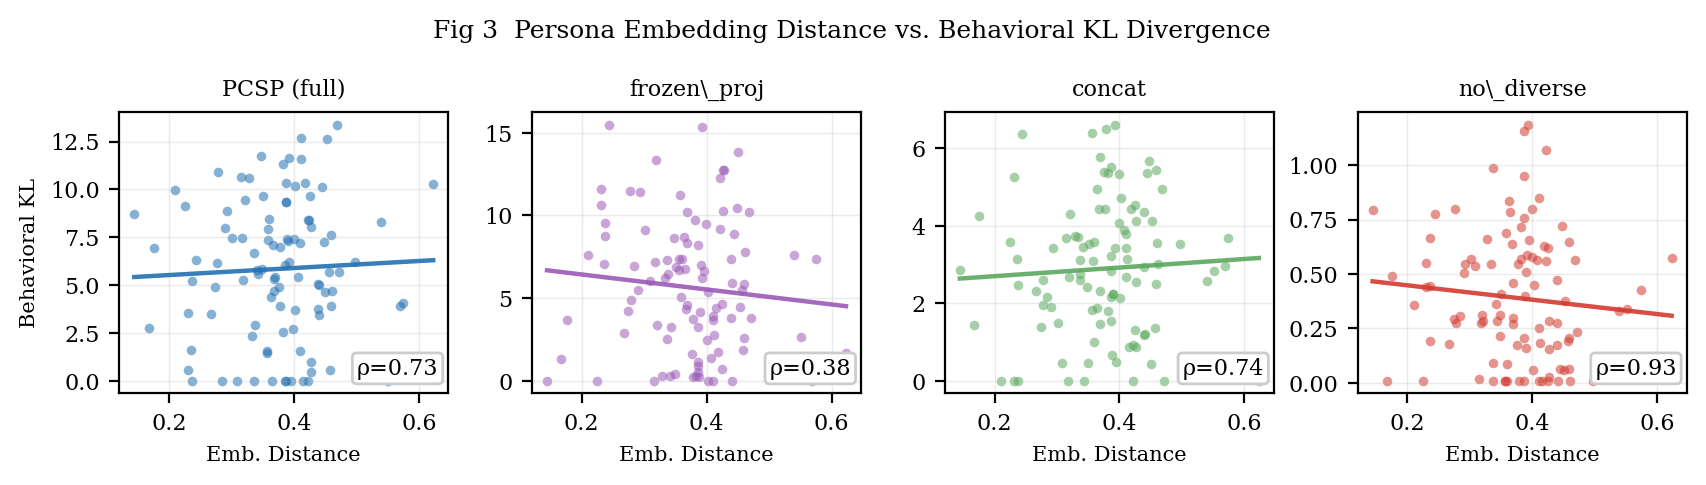
\includegraphics[width=0.98\linewidth]{figures/fig3_kl_scatter.png}
  \caption{
    \textbf{Persona embedding distance vs.\ behavioral KL divergence.}
    Each point is a persona pair; the line shows the linear trend.
    \PCSP{} (full) achieves strong alignment ($\rho\!=\!0.728$);
    removing the LoRA projection (\texttt{frozen\_proj}) halves it to 0.384.
    \texttt{no\_diverse} shows artificially high $\rho$ due to near-zero KL.
  }
  \label{fig:kl_scatter}
\end{figure}

Figure~\ref{fig:kl_scatter} plots pairwise behavioral KL divergence against
persona embedding cosine distance for \PCSP{} (full) and ablations.
\PCSP{} shows a strong monotone trend ($\rho\!=\!0.728$, $p\!<\!10^{-17}$):
more dissimilar personas produce more dissimilar behaviors.
frozen\_proj loses this alignment ($\rho\!=\!0.384$), confirming the role of
the LoRA projection in bridging LLM and behavior spaces.

% ---------------------------------------------------------------
\section{Conclusion}
\label{sec:conclusion}

We presented \PCSP{}, the first framework that grounds free-form natural
language persona descriptions into a single shared RL policy, enabling
zero-shot generation of behaviorally distinct yet persona-consistent NPCs at
constant inference cost.
Key findings: (1) diversity loss is the most critical component for preventing
behavioral collapse; (2) FiLM conditioning outperforms simple concatenation in
behavioral range; (3) LoRA projection is necessary to align LLM semantic
structure with behavior space; (4) the system generalizes to unseen personas
at 22$\times$ the speed of LLM-as-policy baselines.

\paragraph{Limitations and future work.}
Mini-Inzoi's 6$\times$6 grid is intentionally minimal; scaling to richer
environments (e.g., Melting Pot) is a natural next step.
Dynamic personas (mood evolution over time) and hierarchical persona
representations are planned extensions.
Human evaluation (Prolific, $n\!=\!30$) is ongoing and will be included in the
final version.

% ---------------------------------------------------------------
\paragraph{Acknowledgements.}
The authors used an NVIDIA RTX 6000 Ada GPU for all experiments.

% ---------------------------------------------------------------
\bibliographystyle{plain}
\bibliography{refs}

\end{document}
